\lecture{Caracterização de Sinais e Sistemas}{lec_carac}

\begin{frame}
	\begin{block}{\centering\large\bfseries Parte 2}
		\centering\large\insertpart
	\end{block}
\end{frame}


\section{Introdução}

\begin{frame}
	\frametitle{Introduçao}

	\begin{itemize}
	 \item Sinais podem ser caracterizados como:
	  \begin{itemize}
	   \item Aleatório vs. determinístico, discreto vs. contínuo no tempo, amplitude discreta vs. contínua, passa-baixa vs. passa-faixa, energia finita vs. infinita, potência média finita vs. infinita, etc.
	  \end{itemize}
	  \item Neste capítulo:
	  \begin{itemize}
	   \item Caracterização de sinais e sistemas comumente encontrados na transmissão de informação digital sobre um canal de comunicação.
	   \item Representação de várias formas de sinais modulados digitalmente e suas características espectrais.
	  \end{itemize}
	\end{itemize}

\end{frame}


\section{Representação de sinais e sistemas em banda passante}

\begin{frame}
	\frametitle{Representação de sinais e sistemas em banda passante}

	\begin{itemize}
	 \item Transmissão de sinais digitais $\Rightarrow$ modulação de portadora
	 \item Canal limitado em largura de banda: 
	\begin{itemize}
	 \item Double sideband (DSB): intervalo de frequências centradas em torno da portadora
	 \item Single sideband (SSB): intervalo de frequências adjacentes à portadora
	 \end{itemize}
	\item Sinais e sistemas de banda estreita (narrowband)
	\begin{itemize}
	 \item Largura de banda muito menor que a frequência da portadora
	 \end{itemize}
	  \item Transmissão e recepção de sinais em banda passante:
	\begin{itemize}
	 \item Envolve translações de frequência
	 \end{itemize}
	 \item Sinais e canais passa-baixa equivalentes:
	\begin{itemize}
	 \item Não há perda de generalidade
	  \item Conveniência matemática
	  \item Independentes da frequência de portadora e bandas de canais
	 \end{itemize}
	\end{itemize}

\end{frame}

\begin{frame}
	\frametitle{Representação de sinais em banda passante}

	\begin{itemize}
	 \item Sinal $s(t)$ com conteúdo em frequência concentrado em uma banda estreita de frequências em torno de $f_c$
	\end{itemize}
	\begin{figure}[t]
	  \begin{center}
	    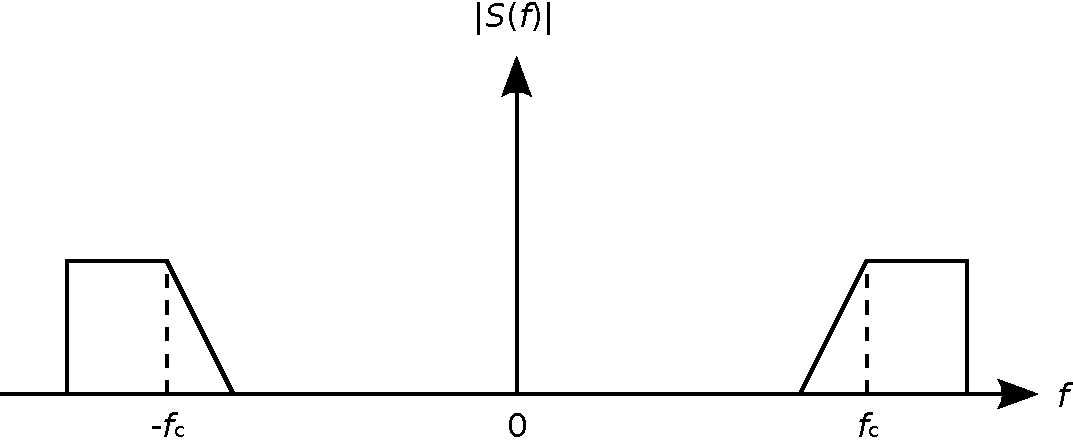
\includegraphics[width=0.5\columnwidth]{figs/4-1-1}
	  \end{center}
	\end{figure}
	\begin{itemize}
	 \item Sinal contendo as frequências positivas:
	\end{itemize}
	\begin{align*}
	      S_+(f) &= 2u(f)S(f) \\
	      s_+(t) &= \int_{-\infty}^{\infty}S_+(f)e^{j2\pi ft}df \\
	      &= F^{-1}[2u(f)] \ast F^{-1}[S(f)]
	\end{align*}

\end{frame}

\begin{frame}
	\frametitle{Representação de sinais em banda passante}

	\begin{itemize}
	 \item $s_+(t)$ é o sinal analítico ou pré-envoltória de $s(t)$
	 \item Considerando que $F^{-1}[S(f)] = s(t)$ e $F^{-1}[2u(f)] = \delta(t) + j/\pi t$
	\end{itemize}
	\begin{align*}
	    s_+(t) &= \left[ \delta(t) + \frac{j}{\pi t} \right] \ast s(t) \\
		  &= s(t) + j \underbrace{\frac{1}{\pi t}\ast s(t)}_{\hat{s}(t)}
	\end{align*}
	\begin{itemize}
	 \item $\hat{s}(t)$ pode ser visto como a saída do filtro de resposta ao impulso $h(t) = 1/\pi t$ quando excitado por $s(t)$. Transformada de Hilbert:
	\end{itemize}
	\begin{align*}
	    H(f) = \int_{-\infty}^{\infty} h(t) e^{-j2\pi ft}dt = \frac{1}{\pi} \int_{-\infty}^{\infty} \frac{1}{t} e^{-j2\pi ft}dt = \begin{cases} -j & f>0 \\ 0 & f = 0 \\ j & f < 0 \end{cases}
	\end{align*}
\end{frame}

\begin{frame}
	\frametitle{Representação de sinais em banda passante}

	\begin{itemize}
	 \item Efeito: deslocamento de fase de 90$^\mathrm{o}$ para todas as frequências de $s(t)$
	  \item Equivalente passa-baixa de $S_+(f)$: $S_l(f) = S_+(f+f_c)$
	  \item No domínio do tempo temos
	\end{itemize}
	\begin{align*}
	      s_l(t) &= s_+(t) e^{-j2\pi f_c t} = [s(t) + j \hat{s}(t)]e^{-j2\pi f_c t}
	\end{align*}
	\begin{itemize}
	 \item Considerando que $s_l(t) = x(t) + jy(t)$, podemos isolar $s(t)$ e $\hat{s}(t)$ como função das componentes do equivalente passa-baixa:
	\end{itemize}
	\begin{align*}
	      s(t) + j \hat{s}(t) &= s_l(t) e^{j2\pi f_c t} = [x(t) + jy(t)] e^{j2\pi f_c t} \\
	      s(t) &= x(t) \cos 2\pi f_c t - y(t) \sin 2\pi f_c t \\
	      \hat{s}(t) &= x(t) \sin 2\pi f_c t + y(t) \cos 2\pi f_c t \\
	\end{align*}

\end{frame}

\begin{frame}
	\frametitle{Representação de sinais em banda passante}

	\begin{itemize}
	 \item $x(t)$ e $y(t)$: componentes em quadratura do sinal em banda passante
	  \item $s_l(t)$: envoltória complexa do sinal real $s(t)$
	  \item Outras representações para o sinal em banda passante:
	\end{itemize}
	\begin{align*}
	    s(t) &= \mathrm{Re}\{[x(t) + jy(t)]e^{j2\pi f_c t}\} = \mathrm{Re}\{s_l(t) e^{j2\pi f_c t}\} \\
	    s(t) &= \mathrm{Re}\{a(t) e^{j[2\pi f_c t + \theta(t)]}\} = a(t) \cos [ 2\pi f_c t + \theta(t) ] \\
	\end{align*}
	\begin{itemize}
	 \item $a(t)$ e $\theta(t)$ são a envoltória e fase do sinal em banda passante
	 \item Temos que $s_l(t) = a(t) e^{j\theta(t)}$, $a(t) = \sqrt{x^2(t) + y^2(t)}$ e $\theta(t) = \tan^{-1} [y(t)/x(t)]$
	\end{itemize}

\end{frame}

\begin{frame}
	\frametitle{Representação de sinais em banda passante}

	\begin{itemize}
	 \item Calculando a transformada de Fourier de $s(t)$:
	\end{itemize}
	\begin{align*}
	    S(f) &= \int_{-\infty}^{\infty} s(t) e^{-j2\pi f t} dt = \int_{-\infty}^{\infty} \{ \mathrm{Re}[s_l(t) e^{j2\pi f_c t}] \} e^{-j2\pi f t} dt \\
	    &= \frac{1}{2} \int_{-\infty}^{\infty} [ s_l(t) e^{j2\pi f_c t} + s_l^*(t) e^{-j2\pi f_c t} ] e^{-j2\pi f t} dt \\
	    &= \frac{1}{2} [ S_l(f -f_c) + S_l^*(-f -f_c) ]
	\end{align*}
	\begin{itemize}
	 \item Relação básica entre o espectro do sinal equivalente passa-baixa e o espectro do sinal em banda passante
	\end{itemize}

\end{frame}

\begin{frame}
	\frametitle{Representação de sinais em banda passante}

	\begin{itemize}
	 \item Energia do sinal:
	\end{itemize}
	\begin{align*}
	    \mathcal{E} &= \int_{-\infty}^{\infty} s^2(t) dt = \int_{-\infty}^{\infty} \{ \mathrm{Re}[s_l(t)e^{j2\pi f_c t}] \}^2 dt \\
	    &= \frac{1}{2} \int_{-\infty}^{\infty} |s_l(t)|^2 dt + \color{red}{\frac{1}{2} \int_{-\infty}^{\infty} |s_l(t)|^2 \cos [4\pi f_c t + 2\theta(t)] dt}
	\end{align*}
	\begin{itemize}
	  \item Assumindo que $s(t)$ possui banda estreita, tem-se que a segunda integral possui um valor muito menor que a primeira, podendo ser desconsiderada
	  \item Pode-se afirmar que a energia do sinal equivalente passa-baixa corresponde, na prática, à energia do sinal em banda passante
	\end{itemize}

\end{frame}

\begin{frame}
	\frametitle{Representação de sinais em banda passante}

	\begin{figure}[t]
	  \begin{center}
	    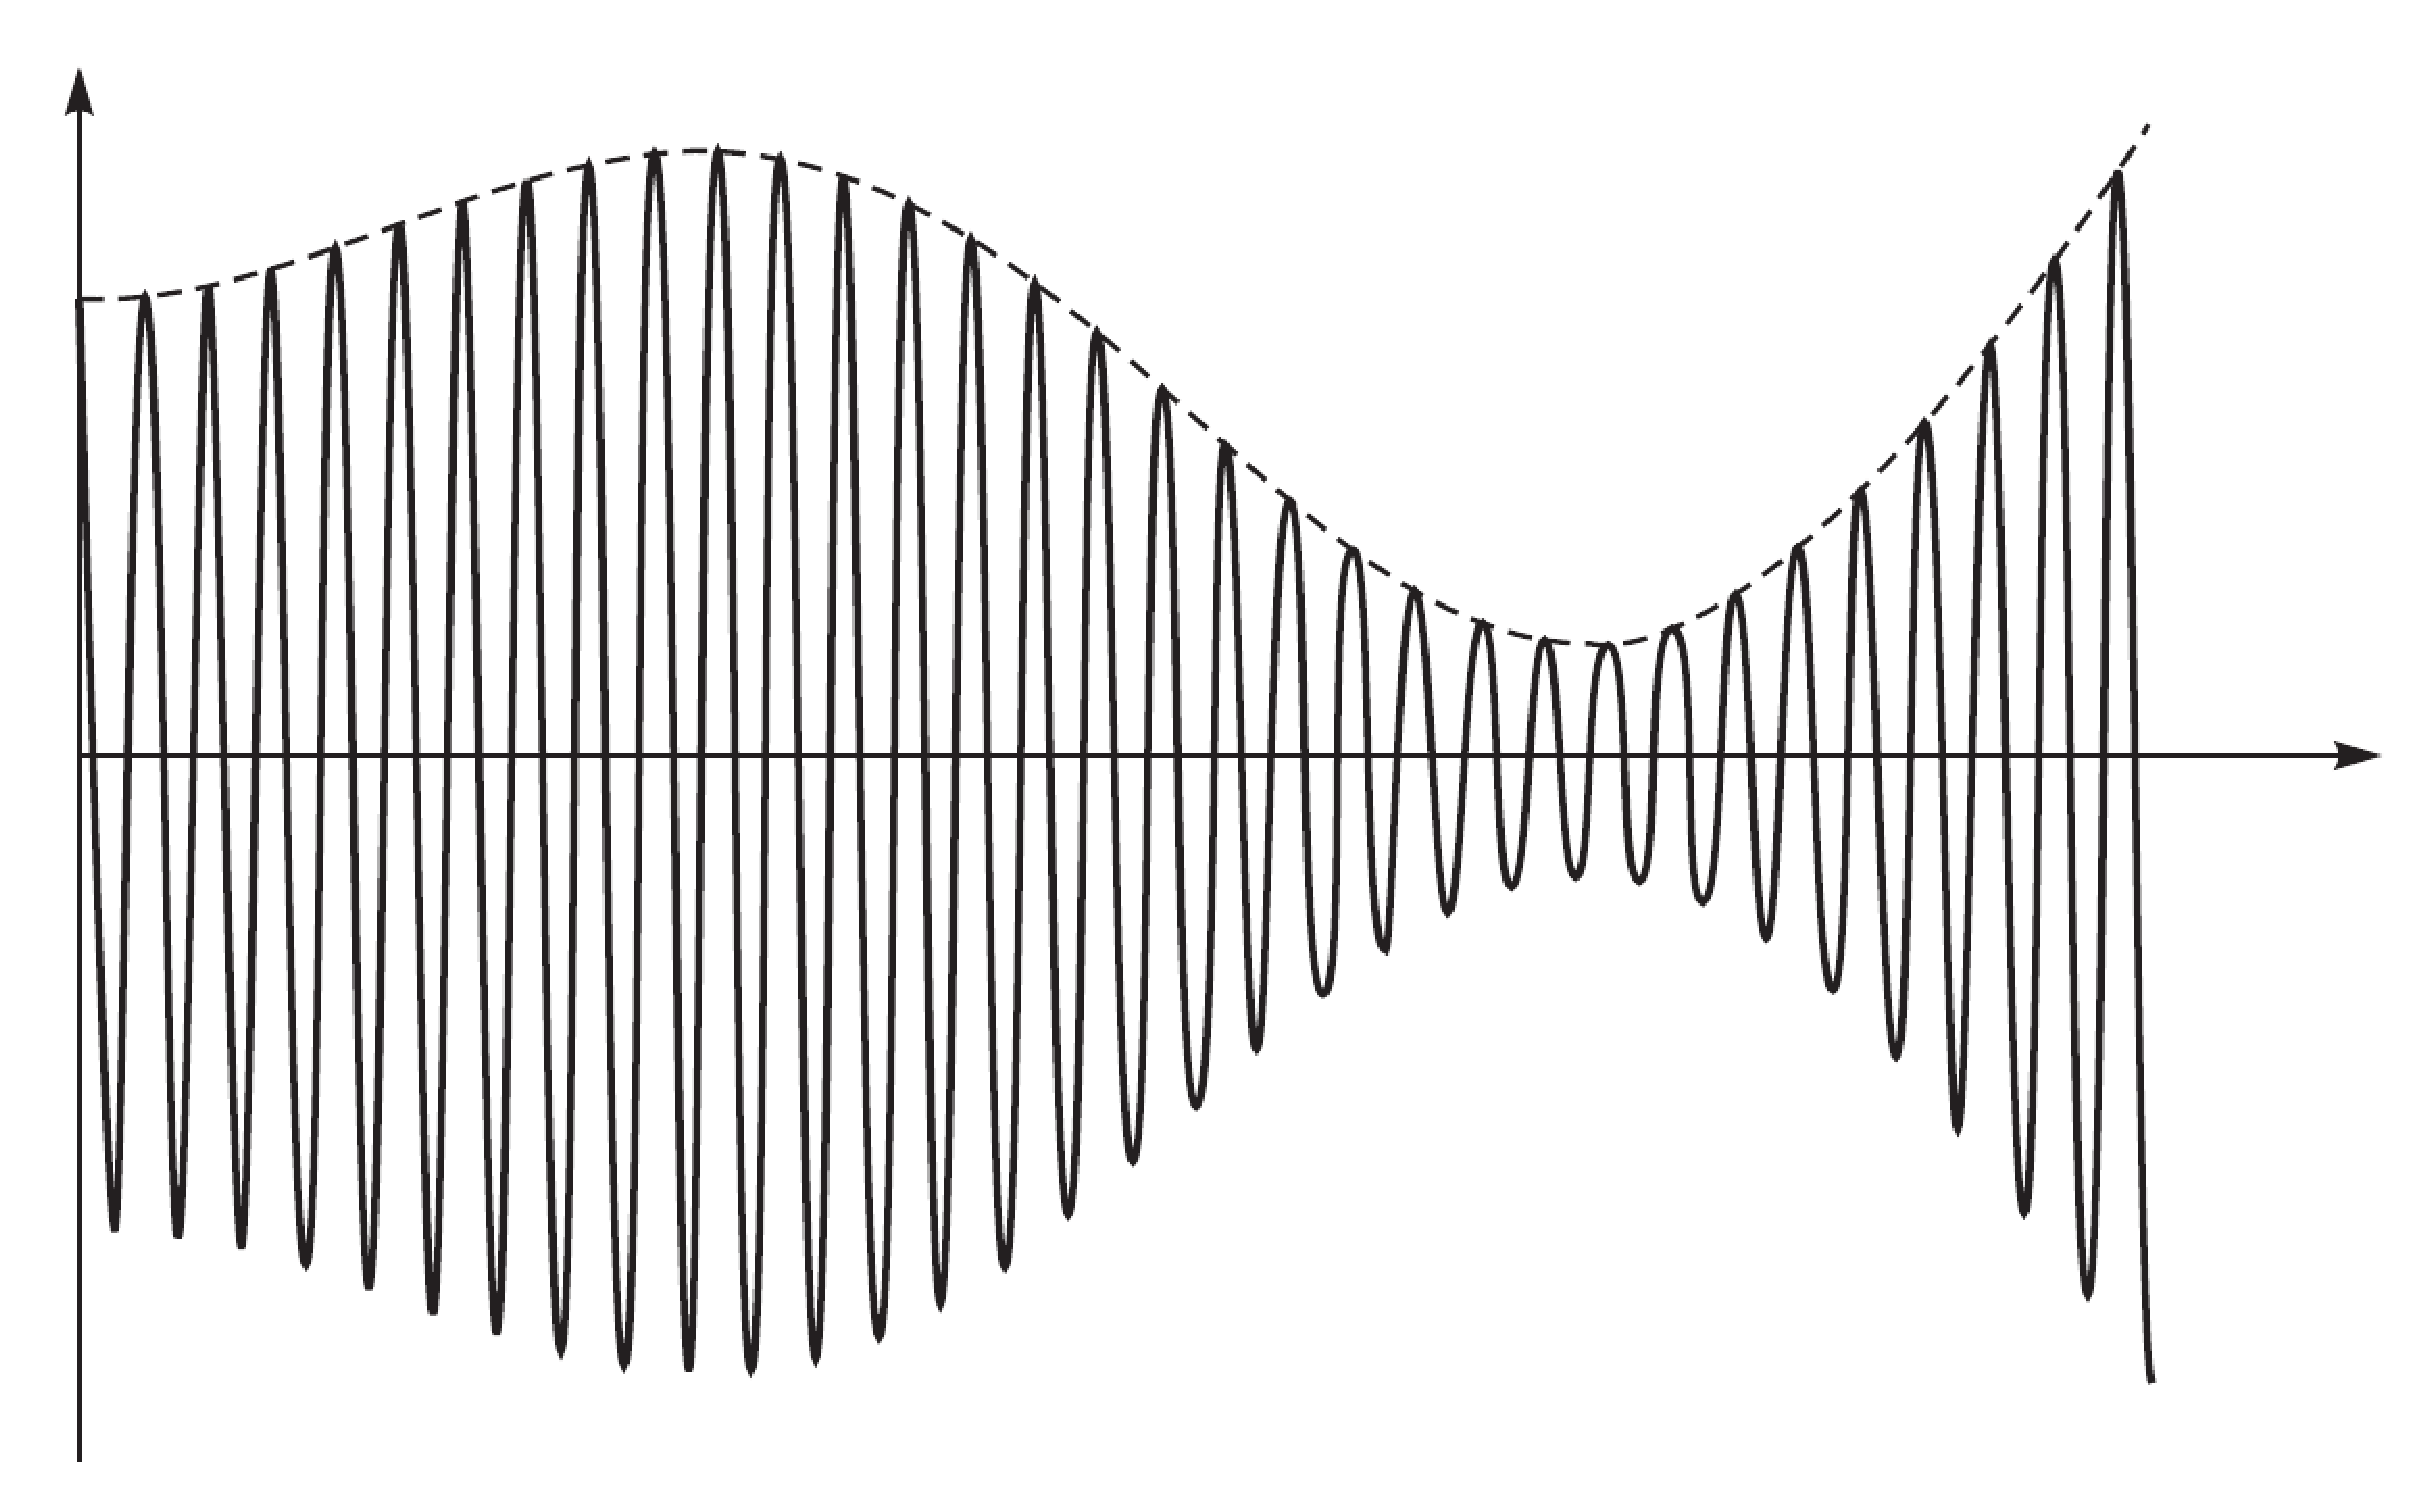
\includegraphics[width=0.5\columnwidth]{figs/fig02-01-04}
	  \end{center}
	\end{figure}

	\begin{itemize}
	  \item Para fins práticos pode-ser afirmar que, a energia do sinal em banda passante $s(t)$, expressa em termos do sinal equivalente passa-baixa $s_l(t)$, é dada por:
	\end{itemize}
	\begin{equation*}
	      \mathcal{E} = \frac{1}{2} \int_{\infty}^{\infty} |s_l(t)|^2 dt
	\end{equation*}


\end{frame}

\begin{frame}
	\frametitle{Representação de um sistema linear em banda passante}

	\begin{itemize}
	  \item Um filtro ou um sistema linear pode ser descrito por $h(t)$ ou $H(f)$.
	  \item Assumindo que $h(t)$ é real:
	  	\begin{equation*}
	      H^*(-f) = H(f)
	\end{equation*}
	  \item Considere que:
	\begin{align*}
	      H_l(f-f_c) &= \begin{cases}
				H(f) , &f > 0 \\
			        0, &f < 0 
	                    \end{cases} \\
	      H_l^*(-f-f_c) &= \begin{cases}
				0, &f > 0 \\
			        H^*(-f), &f < 0 
	                    \end{cases}
	\end{align*}
	 \item Então:
	\begin{equation*}
	    H(f) = H_l(f-f_c) + H_l^*(-f-f_c)
	\end{equation*}
	\end{itemize}


\end{frame}

\begin{frame}
	\frametitle{Resposta de um sistema em banda passante a um sinal em banda passante}

	\begin{itemize}
	  \item A resposta de um sistema em banda passante a um sinal de entrada em banda passante pode ser obtida a partir dos equivalentes passa-baixa do sinal de entrada e da resposta ao impulso do sistema.
	  \begin{figure}[t]
	  \begin{center}
	    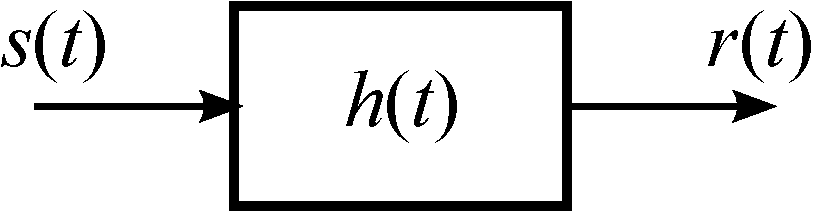
\includegraphics[width=0.3\columnwidth]{figs/system}
	  \end{center}
	\end{figure}
	  \item A saída do sistema também é um sinal em banda passante e pode ser representada por: $r(t) = \mathrm{Re}[r_l(t)e^{j2\pi f_c t}]$
	 \begin{small}\begin{align*}
	      R(f) &= S(f)H(f) \\
	      &= \frac{1}{2}[S_l(f-f_c) + S_l^*(-f-f_c)][H_l(f-f_c) + H_l^*(-f-f_c)] \\
	      &= \frac{1}{2}[S_l(f-f_c)H_l(f-f_c) + S_l^*(-f-f_c)H_l^*(-f-f_c)] \\
	      &= \frac{1}{2}[R_l(f-f_c) + R_l^*(-f-f_c)]
	\end{align*}	            \end{small}
	\end{itemize}


\end{frame}

\begin{frame}
	\frametitle{Representação de processos estocásticos estacionários em banda passante}

	\begin{itemize}
	  \item Representação é extendida para funções amostra de um processo estocástico estacionário em banda passante.
	  \item Derivação das relações entre as funções de correlação e o espectro de potência dos sinais em banda passante e do equivalente passa-baixa.
	  \item Processo estocástico do ruído
	  \begin{itemize}
	   \item $n(t)$: função amostra de um processo WSS com média zero e DEP $\Phi_{nn}(f)$
	   \item DEP limitada a um intervalo de frequências em torno de $f_c$
	   \item Processo em banda passante de banda estreita: largura da DEP $\gg f_c$
	   \item Representação do ruído:
	   \begin{align*}
		n(t) &= a(t)\cos[2\pi f_c t + \theta(t)] \\
		&= x(t)\cos 2\pi f_c t - y(t) \sin 2\pi f_c t \\
		&= \mathrm{Re}[z(t)e^{j2\pi f_c t}]
	   \end{align*}

	  \end{itemize}

	\end{itemize}

\end{frame}

\begin{frame}
	\frametitle{Representação de processos estocásticos estacionários em banda passante}

	\begin{itemize}
		\item Se $n(t)$ possui média zero, então $x(t)$ e $y(t)$ também têm média zero.
		\item A estacionariedade de $n(t)$ implica nas seguintes propriedades:
		\begin{align*}
			\phi_{xx}(\tau) &= \phi_{yy}(\tau) \\
			\phi_{xy}(\tau) &= -\phi_{yx}(\tau) 
		\end{align*}
		\item Função de autocorrelação do processo $n(t)$:
		\begin{equation*}
			\phi_{nn}(\tau) = \phi_{xx}(\tau)\cos 2\pi f_c \tau - \phi_{yx}(\tau)\sin 2\pi f_c \tau
		\end{equation*}
		\item Função de autocorrelação do processo equivalente passa-baixa $z(t) = x(t) + jy(t)$:
		\begin{align*}
			\phi_{zz}(\tau) &= \frac{1}{2} \expec[z^*(t) z(t+\tau)] = \phi_{xx}(\tau) + j\phi_{yx}(\tau) \\
			\phi_{nn}(\tau) &= \mathrm{Re}[\phi_{zz}(\tau)e^{j2\pi f_c \tau}]
		\end{align*}
	\end{itemize}

\end{frame}

\begin{frame}
	\frametitle{Representação de processos estocásticos estacionários em banda passante}

	\begin{itemize}
		\item Densidade espectral de potência do processo $n(t)$:
		\begin{small}\begin{equation*}
			\Phi_{nn}(f) = \int_{-\infty}^{\infty}\{\mathrm{Re}[\phi_{zz}(\tau)e^{j2\pi f_c \tau}]\}e^{-j2\pi f \tau} d\tau = \frac{1}{2}[\Phi_{zz}(f-f_c)+\Phi_{zz}(-f-f_c)]
		\end{equation*}		               \end{small}
 		\item Uma vez que $\phi_{zz}(\tau) = \phi_{zz}^*(-\tau)$,  então $\Phi_{zz}(f)$ é real.
		\item A partir das relações:
		\vspace{-0.1cm}\begin{align*}
			\phi_{xy}(\tau) &= -\phi_{yx}(\tau) \\
			\phi_{yx}(\tau) &= \phi_{xy}(-\tau)
		\end{align*}
 		\item Temos que $\phi_{xy}(\tau) = -\phi_{xy}(-\tau)$,  ou seja, $\phi_{xy}(\tau)$ é uma função ímpar.
		\item Consequentemente, $\phi_{xy}(0) = 0$, o que significa que $x(t)$ e $y(t)$ são descorrelacionados para $\tau=0$.
		\item Caso $\phi_{xy}(\tau) = 0$ para todo $\tau$,  então $\phi_{zz}(\tau)$ é real e $\Phi_{zz}(f) = \Phi_{zz}(-f)$.
	\end{itemize}

\end{frame}

\begin{frame}
	\frametitle{Representação de processos estocásticos estacionários em banda passante}

	\begin{itemize}
		\item Caso em que $n(t)$ é um processo Gaussiano:
		\begin{itemize}
			\item Componentes em quadratura $x(t)$ e $y(t+\tau)$ são conjuntamente Gaussianas.
			\item Para $\tau=0$ são independentes e possuem densidade conjunta:
			\begin{equation*}
				p(x,y) = \frac{1}{2\pi \sigma^2}e^{-(x^2+y^2)/2\sigma^2}
			\end{equation*}
			\item Onde $\sigma^2 = \phi_{xx}(0) = \phi_{yy}(0) = \phi_{nn}(0)$.
		\end{itemize}
	\end{itemize}

\end{frame}

\begin{frame}
	\frametitle{Representação de processos estocásticos estacionários em banda passante}

	\begin{itemize}
		\item Representação do ruído branco:
		\begin{itemize}
			\item DEP constante sobre todo o espectro de frequência.
			\item Ruído branco de banda estreita: assume-se que o ruído passou por um filtro e está limitado à banda do sinal.
			\item DEP e autocorrelação do equivalente passa-baixa $z(t)$:
			\begin{align*}
				\Phi_{zz}(f) &= \begin{cases}
							N_0 &\quad (|f| \leq B/2) \\
							0 &\quad (|f| > B/2)
				               \end{cases} \\
				\phi_{zz}(\tau) &= N_0 \frac{\sin \pi B \tau}{\pi\tau} \; ; \quad \lim_{B \to \infty} \phi_{zz}(\tau) = N_0\delta(\tau)
			\end{align*}
			\item Como a DEP é simétrica em torno de $f=0$, então $\phi_{yx}=0$ para todo $\tau$ e $\phi_{zz}(\tau)=\phi_{xx}(\tau)=\phi_{yy}(\tau)$.
			\item Ou seja, $x(t)$ e $y(t)$ são sempre descorrelacionados e as autocorrelações de $z(t)$,  $x(t)$ e $y(t)$ são iguais.
		\end{itemize}

	\end{itemize}

\end{frame}


%--------------------

\section{Representação em espaço de sinais}

\begin{frame}
	\frametitle{Conceitos de espaço vetorial}

	\begin{itemize}
	 \item Um vetor $\vv$ em um espaço $n$-dimensional é caracterizado por suas $n$ componentes $[v_1 \; v_2 \; \ldots \; v_n]$
	  \item Também pode ser representado como uma combinação linear de vetores unitários: $\vv = \sum\limits_{i=1}^n v_i \, \ve_i$, para $1 \leq i \leq n$
	  \item Onde $v_i$ é a projeção de $\vv$ em $\ve_i$
	  \item O produto interno de dois vetores $n$-dimensionais é dado por: $\vv_1 \cdot \vv_2 = \sum\limits_{i=1}^n v_{1i} \, v_{2i}$
	  \item Condição de ortogonalidade entre dois vetores: $\vv_1 \cdot \vv_2 = 0$
	  \item Um conjunto de $m$ vetores $\vv_k$, $1\leq k \leq m$, é ortogonal se: $\vv_i \cdot \vv_j = 0$ para todo $(i,j) \in \{1, \ldots, m\}$ e $i \neq j$
	\end{itemize}

\end{frame}


\begin{frame}
	\frametitle{Conceitos de espaço vetorial}

	\begin{itemize}
	 \item Norma de um vetor: $||\vv|| = (\vv \cdot \vv)^{1/2} = \sqrt{\sum\limits_{i=1}^n v_i^2}$
	  \item Conjunto de vetores ortonormais: conjunto de vetores ortogonais onde cada vetor possui norma unitária
	  \item Conjunto de vetores LI: nenhum vetor do conjunto pode ser expresso como uma combinação linear dos outros vetores
	  \item Desigualdade triangular: $||\vv_1 + \vv_2|| \leq ||\vv_1|| + ||\vv_2||$. Igualdade somente para $\vv_1$ e $\vv_2$ colineares, ou seja, $\vv_1 = a\vv_2$
	  \item Desigualdade de Cauchy-Schwarz: $|\vv_1 \cdot \vv_2| \leq ||\vv_1 || \; ||\vv_2 ||$. Igualdade somente para $\vv_1 = a\vv_2$
	  \item Norma ao quadrado da soma de vetores: $||\vv_1 + \vv_2||^2 = ||\vv_1||^2 + ||\vv_2||^2 + 2 \vv_1 \cdot \vv_2$
	  \item Se $\vv_1$ e $\vv_2$ são ortogonais, então $||\vv_1 + \vv_2||^2 = ||\vv_1||^2 + ||\vv_2||^2$
	\end{itemize}

\end{frame}

\begin{frame}
	\frametitle{Conceitos de espaço vetorial}

	\begin{itemize}
	 \item Transformação linear em um espaço $n$-dimensional: $\vv' = \mA \vv$
	  \item Caso particular em que $\vv' = \lambda \vv$ temos que: $\mA \vv = \lambda \vv$
 	  \item $\vv$ é chamado de autovetor da transformação e $\lambda$ é o autovalor correspondente
	  \item Procedimento de Gram-Schmidt: construção de um conjunto de vetores ortonormais a partir de um conjunto de vetores $n$-dimensionais $\vv_i$
	\end{itemize} \vspace{-0.4cm}
	\begin{align*}
	      \vu_1 &= \vv_1 / ||\vv_1|| \\
	      \vu_2' &= \vv_2 - (\vv_2 \cdot \vu_1)\vu_1 \quad , \qquad \vu_2 = \vu_2' / ||\vu_2'|| \\
	      \vu_3' &= \vv_3 - (\vv_3 \cdot \vu_1)\vu_1 - (\vv_3 \cdot \vu_2)\vu_2 \quad , \qquad \vu_3 = \vu_3' / ||\vu_3'|| \\
	      \ldots
	\end{align*} \vspace{-0.5cm}
	\begin{itemize} 
	 \item Obtém-se um conjunto de $n_1$ vetores onde, em geral, $n_1 \leq n$
	\end{itemize}

\end{frame}

\begin{frame}
	\frametitle{Conceitos de espaço de sinais}

	\begin{itemize}
	  \item Analogia entre vetores e conjunto de sinais definidos em intervalo $[a,b]$
	  \item Sejam os sinais complexos $x_1(t)$ e $x_2(t)$, o seu produto interno é: $<x_1(t),x_2(t)> = \int_a^b x_1(t) x_2^*(t) dt$
	  \item A norma de um sinal é definida como: $||x(t)|| = \left( \int_a^b |x(t)|^2 dt \right)^{1/2}$
	  \item Definições de conjunto ortonormal e independência linear análogas ao caso vetorial
	  \item Desigualdade triangular: $||x_1(t) + x_2(t)|| \leq ||x_1(t)|| + ||x_2(t)||$
	  \item Desigualdade de Cauchy-Schwarz: 
	  \begin{equation*}
		    \left|\int_a^b x_1(t) x_2^*(t) dt \right| \leq \left|\int_a^b |x_1(t)|^2 dt \right|^{1/2} \left|\int_a^b |x_2(t)|^2 dt\right|^{1/2}
	  \end{equation*}
	\end{itemize}

\end{frame}

\begin{frame}
	\frametitle{Expansão ortogonal de sinais}

	\begin{itemize}
		\item Sinal $s(t)$ determinístico, real e de energia finita: $\mathcal{E}_s = \int_{-\infty}^{\infty}[s(t)]^2 dt$
		\item Conjunto de funções ortonormais $\{ f_n(t), n=1, 2, \ldots, N\}$ tal que
		\begin{equation*}
			\int_{-\infty}^{\infty} f_n(t)f_m(t) dt = \begin{cases}
									0 &\quad (m\neq n) \\
									1 &\quad (m=n)
			                                          \end{cases}
		\end{equation*}
		\item O sinal $s(t)$ pode ser aproximado por uma combinação linear destas funções:
		\begin{equation*}
			\hat{s}(t) = \sum_{k=1}^{K} s_k f_k(t)
		\end{equation*}
		\item Onde $\{s_k, 1\leq k \leq K\}$ são os coeficientes na aproximação de $s(t)$, sendo o erro de aproximação dado por:
		\begin{equation*}
			e(t) = s(t) - \hat{s}(t)
		\end{equation*}
	\end{itemize}

\end{frame}

\begin{frame}
	\frametitle{Expansão ortogonal de sinais}

	\begin{itemize}
		\item Energia do erro de aproximação:
		\begin{small}\begin{equation*}
			\mathcal{E}_e = \int_{-\infty}^{\infty}[s(t)-\hat{s}(t)]^2 dt = \int_{-\infty}^{\infty}\left[ s(t) - \sum_{k=1}^{K} s_k f_k(t) \right]^2 dt
		\end{equation*}		               \end{small}
		\item Coeficientes ótimos que minimizam a energia do erro podem ser obtidos ao resolver o problema de otimização.
		\item Forma alternativa de encontrar a solução: resultado da teoria da estimação baseado no critério do erro médio quadrático.
		\item O mínimo de $\mathcal{E}_e$ com respeito a $\{s_k\}$ é obtido quando o erro é ortogonal a cada uma das funções da expansão em série, ou seja,
		\begin{small}\begin{equation*}
			\int_{-\infty}^{\infty}\left[ s(t) - \sum_{k=1}^{K} s_k f_k(t) \right]f_n(t) dt = 0,  \quad n=1, 2, \ldots, K
		\end{equation*}		               \end{small}
		\item Como as funções $\{f_n(t)\}$ são ortonormais então temos que:
		\begin{small}\begin{equation*}
			s_n = \int_{-\infty}^{\infty} s(t) f_n(t) dt,  \quad n=1, 2, \ldots, K
		\end{equation*}		               \end{small}
	\end{itemize}
\end{frame}

\begin{frame}
	\frametitle{Expansão ortogonal de sinais}

	\begin{itemize}
		\item Os coeficientes são obtidos ao se projetar $s(t)$ em cada função $\{f_n(t)\}$.
		\item $\hat{s}(t)$ é a projeção de $s(t)$ sobre o espaço de sinal $K$-dimensional definido pelas funções $\{f_n(t)\}$.
		\item O erro quadrático médio de aproximação é dado por:
		\begin{small}\begin{equation*}
			\mathcal{E}_{\text{min}} = \int_{-\infty}^{\infty} e(t) s(t) dt = \int_{-\infty}^{\infty} [s(t)]^2 dt - \int_{-\infty}^{\infty} \sum_{k=1}^{K} s_k f_k(t) s(t) dt = \mathcal{E}_s - \sum_{k=1}^{K} s_k^2
		\end{equation*}		\end{small}
		\item No caso em que $\mathcal{E}_{\text{min}}=0$:
		\begin{equation*}
			\mathcal{E}_s = \sum_{k=1}^{K} s_k^2 = \int_{-\infty}^{\infty} [s(t)]^2 dt \Longrightarrow s(t) = \sum_{k=1}^{K} s_kf_k(t)
		\end{equation*}
		\item O conjunto $\{f_n(t) \}$ é dito \textit{completo} quando todo sinal de energia finito puder ser representado por uma expansão em série para a qual $\mathcal{E}_{\text{min}}=0$.
	\end{itemize}
\end{frame}

\begin{frame}
	\frametitle{Expansão ortogonal de sinais}

	\begin{itemize}
	  \item Procedimento de Gram-Schmidt
	  \begin{itemize}
	   \item Construção de um conjunto de ondas ortonormais a partir de um conjunto finito de sinais de energia $\{s_i(t), i=1,\ldots,M\}$.
	    \end{itemize}
	  \begin{align*}
		    f_1(t) &= \frac{s_1(t)}{||s_1(t)|} \\
		    c_{12} = \int_{-\infty}^{\infty} s_2 f_1(t) dt \, , \qquad f_2(t) &= \frac{s_2(t) - c_{12}f_1(t)}{|| s_2(t) - c_{12}f_1(t) ||} \\
		    &\vdots \\
		    c_{ik} = \int_{-\infty}^{\infty} s_k f_i(t) dt \, , \qquad f_k(t) &= \frac{s_k(t) - \sum_{i=1}^{k-1} c_{ik}f_i(t)}{|| s_k(t) - \sum_{i=1}^{k-1} c_{ik}f_i(t) ||}
	  \end{align*}
	    \item O processo continua até que as $M$ formas de onda tenham sido processadas e $N\leq M$ ondas ortonormais tenham sido construídas.
	    \item Para o caso em que os sinais $s_i(t)$ são LI, temos que $N=M$.
	\end{itemize}

\end{frame}

\begin{frame}
	\frametitle{Expansão ortogonal de sinais}

	\begin{itemize}
	  \item Os $M$ sinais $\{ s_n(t) \}$ podem ser expressos como combinações lineares das funções ortonormais $\{ f_n(t) \}$:
	  \begin{equation*}
		s_k(t) = \sum_{n=1}^{N} s_{kn} f_n(t) , \qquad k=1,\ldots,M 
	  \end{equation*}
	  \item E com relação à energia temos que:
	  \begin{equation*}
	       \mathcal{E}_k = \int_{-\infty}^{\infty} s_k^2(t) dt = \sum_{n=1}^{N} s_{kn}^2 = || \vs_k ||^2
	  \end{equation*}
	  \item Um sinal temporal pode ser representado como um vetor $N$-dimensional:
	  \begin{equation*}
		\vs_k = [ s_{k1} \; s_{k2} \; \ldots \; s_{kN} ]
	  \end{equation*}
	  \item Qualquer sinal pode ser representado geometricamente como um ponto no espaço de sinais definido pelas funções ortonormais $\{ f_n(t) \}$
	\end{itemize}

\end{frame}

\begin{frame}
	\frametitle{Expansão ortogonal de sinais}

	\begin{itemize}
	  \item Caso em que os sinais são definidos em banda passante:
	  \begin{align*}
	      s_m(t) &= \re[s_{lm} e^{j2\pi f_c t}] , \quad m=1,\ldots,M \\
	      \mathcal{E} &= \int_{-\infty}^{\infty} s_m^2(t) dt = \frac{1}{2} \int_{-\infty}^{\infty} |s_{lm}(t)|^2 dt
	  \end{align*}
	  \item Correlação cruzada normalizada:
	   \begin{equation*}
		\frac{1}{\sqrt{\energy_m\energy_k}} \int_{-\infty}^{\infty} s_m(t) s_k(t) dt = \re\left\{ \underbrace{\frac{1}{2\sqrt{\energy_m\energy_k}} \int_{-\infty}^{\infty} s_{lm}(t) s_{lk}^*(t) dt}_{\rho_{km}} \right\}
	   \end{equation*}
	  \item O coeficiente de correlação cruzada real pode ser definido como:
	  \begin{equation*}
		\re(\rho_{km}) = \frac{1}{\sqrt{\energy_m\energy_k}} \int_{-\infty}^{\infty} s_m(t) s_k(t) dt = \frac{\vs_m \cdot \vs_k}{||\vs_m|| ||\vs_k||} = \frac{\vs_m \cdot \vs_k}{\sqrt{\energy_m\energy_k}}
	  \end{equation*}

	\end{itemize}

\end{frame}

\begin{frame}
	\frametitle{Expansão ortogonal de sinais}

	\begin{itemize}
	  \item Distância Euclidiana entre um par de sinais:
	   \begin{align*}
		d_{km}^{(e)} &= ||\vs_m - \vs_k || = \left\{ \int_{-\infty}^{\infty} [ s_m(t) - s_k(t) ]^2 dt \right\}^{1/2} = \\
			     &= \{ \energy_m + \energy_k - 2\sqrt{\energy_m\energy_k} \re(\rho_{km}) \}^{1/2}
	   \end{align*}
	   \item Para o caso em que $\energy_m = \energy_k = \energy$ para todo $m$ e $k$, temos que:
	    \begin{equation*}
		d_{km}^{(e)} = \{2\energy[ 1 - \re(\rho_{km}) ] \}^{1/2}
	    \end{equation*}
	    \item A distância Euclidiana é uma forma alternativa de medir a similaridade dos sinais ou dos vetores correspondentes.
	    \item Exemplo de funções ortonormais em sistemas modulados digitalmente:
	    \begin{equation*}
		f_1(t) = \sqrt{\frac{2}{T}}\cos 2\pi f_c t \qquad f_2(t) = -\sqrt{\frac{2}{T}}\sin 2\pi f_c t
	    \end{equation*}

	\end{itemize}

\end{frame}

\section{Representação de sinais modulados digitalmente}

\begin{frame}
	\frametitle{Representação de sinais modulados digitalmente}

	\begin{itemize}
	  \item Modulador em comunicações digitais:
	  \begin{itemize}
	   \item Mapeia a informação digital em formas de onda analógicas
	   \item Blocos de $k=\log_2 M$ bits são tirados da sequência de informação $\{ a_n \}$
	   \item E são mapeados em uma das $M = 2^k$ formas de onda disponíveis $\{ s_m(t), \; m=1,2,\ldots, M \}$
	  \end{itemize}
	  \item Tipos de mapeamento:
	  \begin{itemize}
	   \item Com memória ou sem memória (dependência de mapeamentos anteriores)
	   \item Linear ou não-linear (princípio da superposição)
	  \end{itemize}
	  \item Formas de onda podem diferir em termos da amplitude, fase, frequência, ou combinação de um ou mais parâmetros.
	  \item Consideração: taxa de dados na entrada do modulador de $R$ bit/s.
	\end{itemize}

\end{frame}

\begin{frame}
	\frametitle{Representação de sinais modulados digitalmente}

	\begin{itemize}
		\item Diagrama de bloco de um esquema de modulação digital sem memória.
	\end{itemize}

	\begin{figure}[t]
	  \begin{center}
	    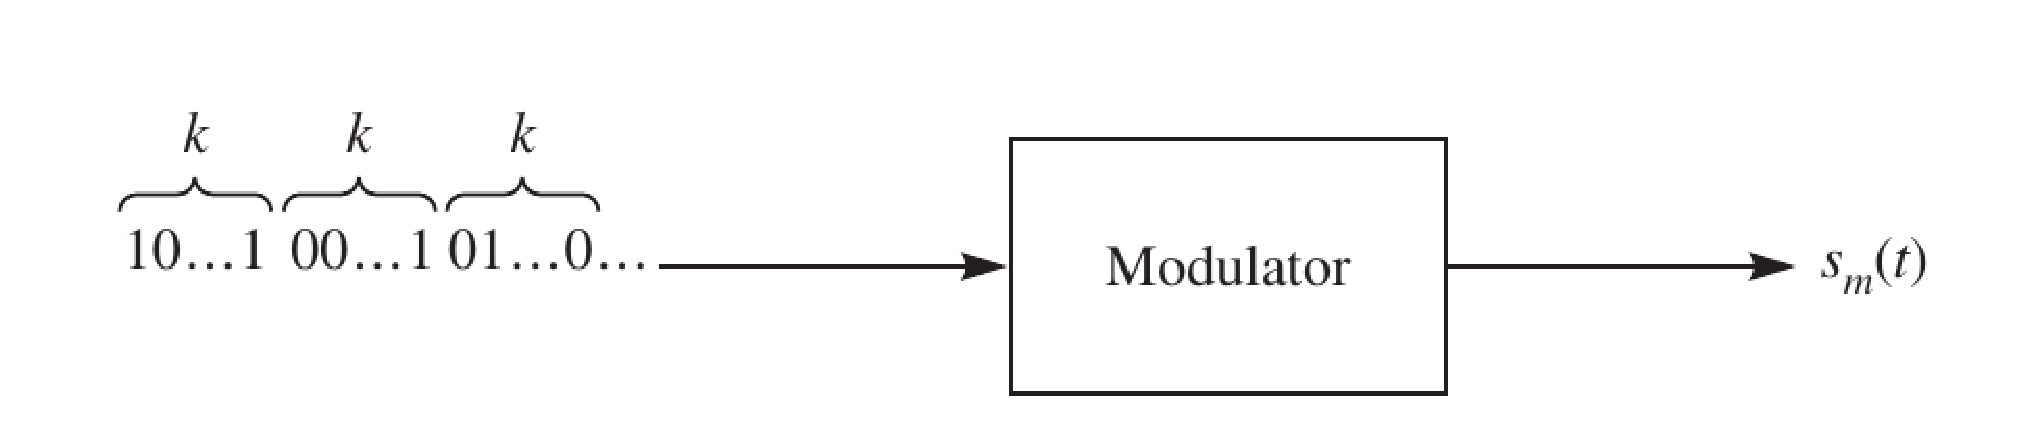
\includegraphics[width=0.7\columnwidth]{figs/mapping}
	  \end{center}
	\end{figure}

\end{frame}

\begin{frame}
	\frametitle{Modulação por amplitude de pulso (PAM)}

	
	   \begin{itemize}
	    \item Amplitude diferencia as formas de onda.
	    \item Formas de onda podem ser representadas como:
	    \begin{align*}
		  s_m(t) &= \re[A_m g(t) e^{j2\pi f_c t}] \\
		  &= A_m g(t) \cos 2\pi f_c t , \quad m=1,2,\ldots, M, \quad 0 \leq t \leq T
	    \end{align*}
	    \item Onde $\{A_m, 1 \leq m \leq M \}$ denota o conjunto de $M=2^k$ possíveis amplitudes, associadas aos blocos de $k$ bits ou \textit{símbolos}.
	    \item Possíveis valores de $A_m$:
	    \begin{equation*}
		A_m = (2m-1-M)d, \quad m=1,2,\ldots,M
	    \end{equation*}
	      \item Onde $2d$ é a distância entre amplitudes de sinais adjacentes.
	      \item O pulso de sinal $g(t)$ é real e sua forma afeta o espectro do sinal transmitido
	   \end{itemize}
	

\end{frame}

\begin{frame}
	\frametitle{Modulação por amplitude de pulso (PAM)}

	\begin{itemize}
	  \item Taxa de símbolos: $R/k$
	  \item Intervalo de bit: $T_b = 1/R$
	  \item Intervalo de símbolo: $T = k/R = kT_b$
	  \item Energia de sinal PAM:
	  \begin{equation*}
	      \mathcal{E}_m = \int_0^T s_m^2(t) dt = \frac{1}{2}A_m^2\int_0^T g^2(t) dt = \frac{1}{2}A_m^2 \mathcal{E}_g
	  \end{equation*}
	   \item Sinais PAM são unidimensionais ($N=1$) e possuem forma geral:
	  \begin{equation*}
	      s_m(t) = s_m f(t)
	  \end{equation*}
	  \item Onde
	      \begin{align*}
		  f(t) &= \sqrt{\frac{2}{\mathcal{E}_g}} g(t) \cos 2\pi f_c t \\
		  s_m &= A_m \sqrt{\energy_g / 2}
	      \end{align*}

	\end{itemize}

\end{frame}

\begin{frame}
	\frametitle{Modulação por amplitude de pulso (PAM)}

	\begin{itemize}
		\item Diagrama de espaço de sinais para sinais digitais PAM.
	\end{itemize}
	
	\begin{figure}[t]
	  \begin{center}
	    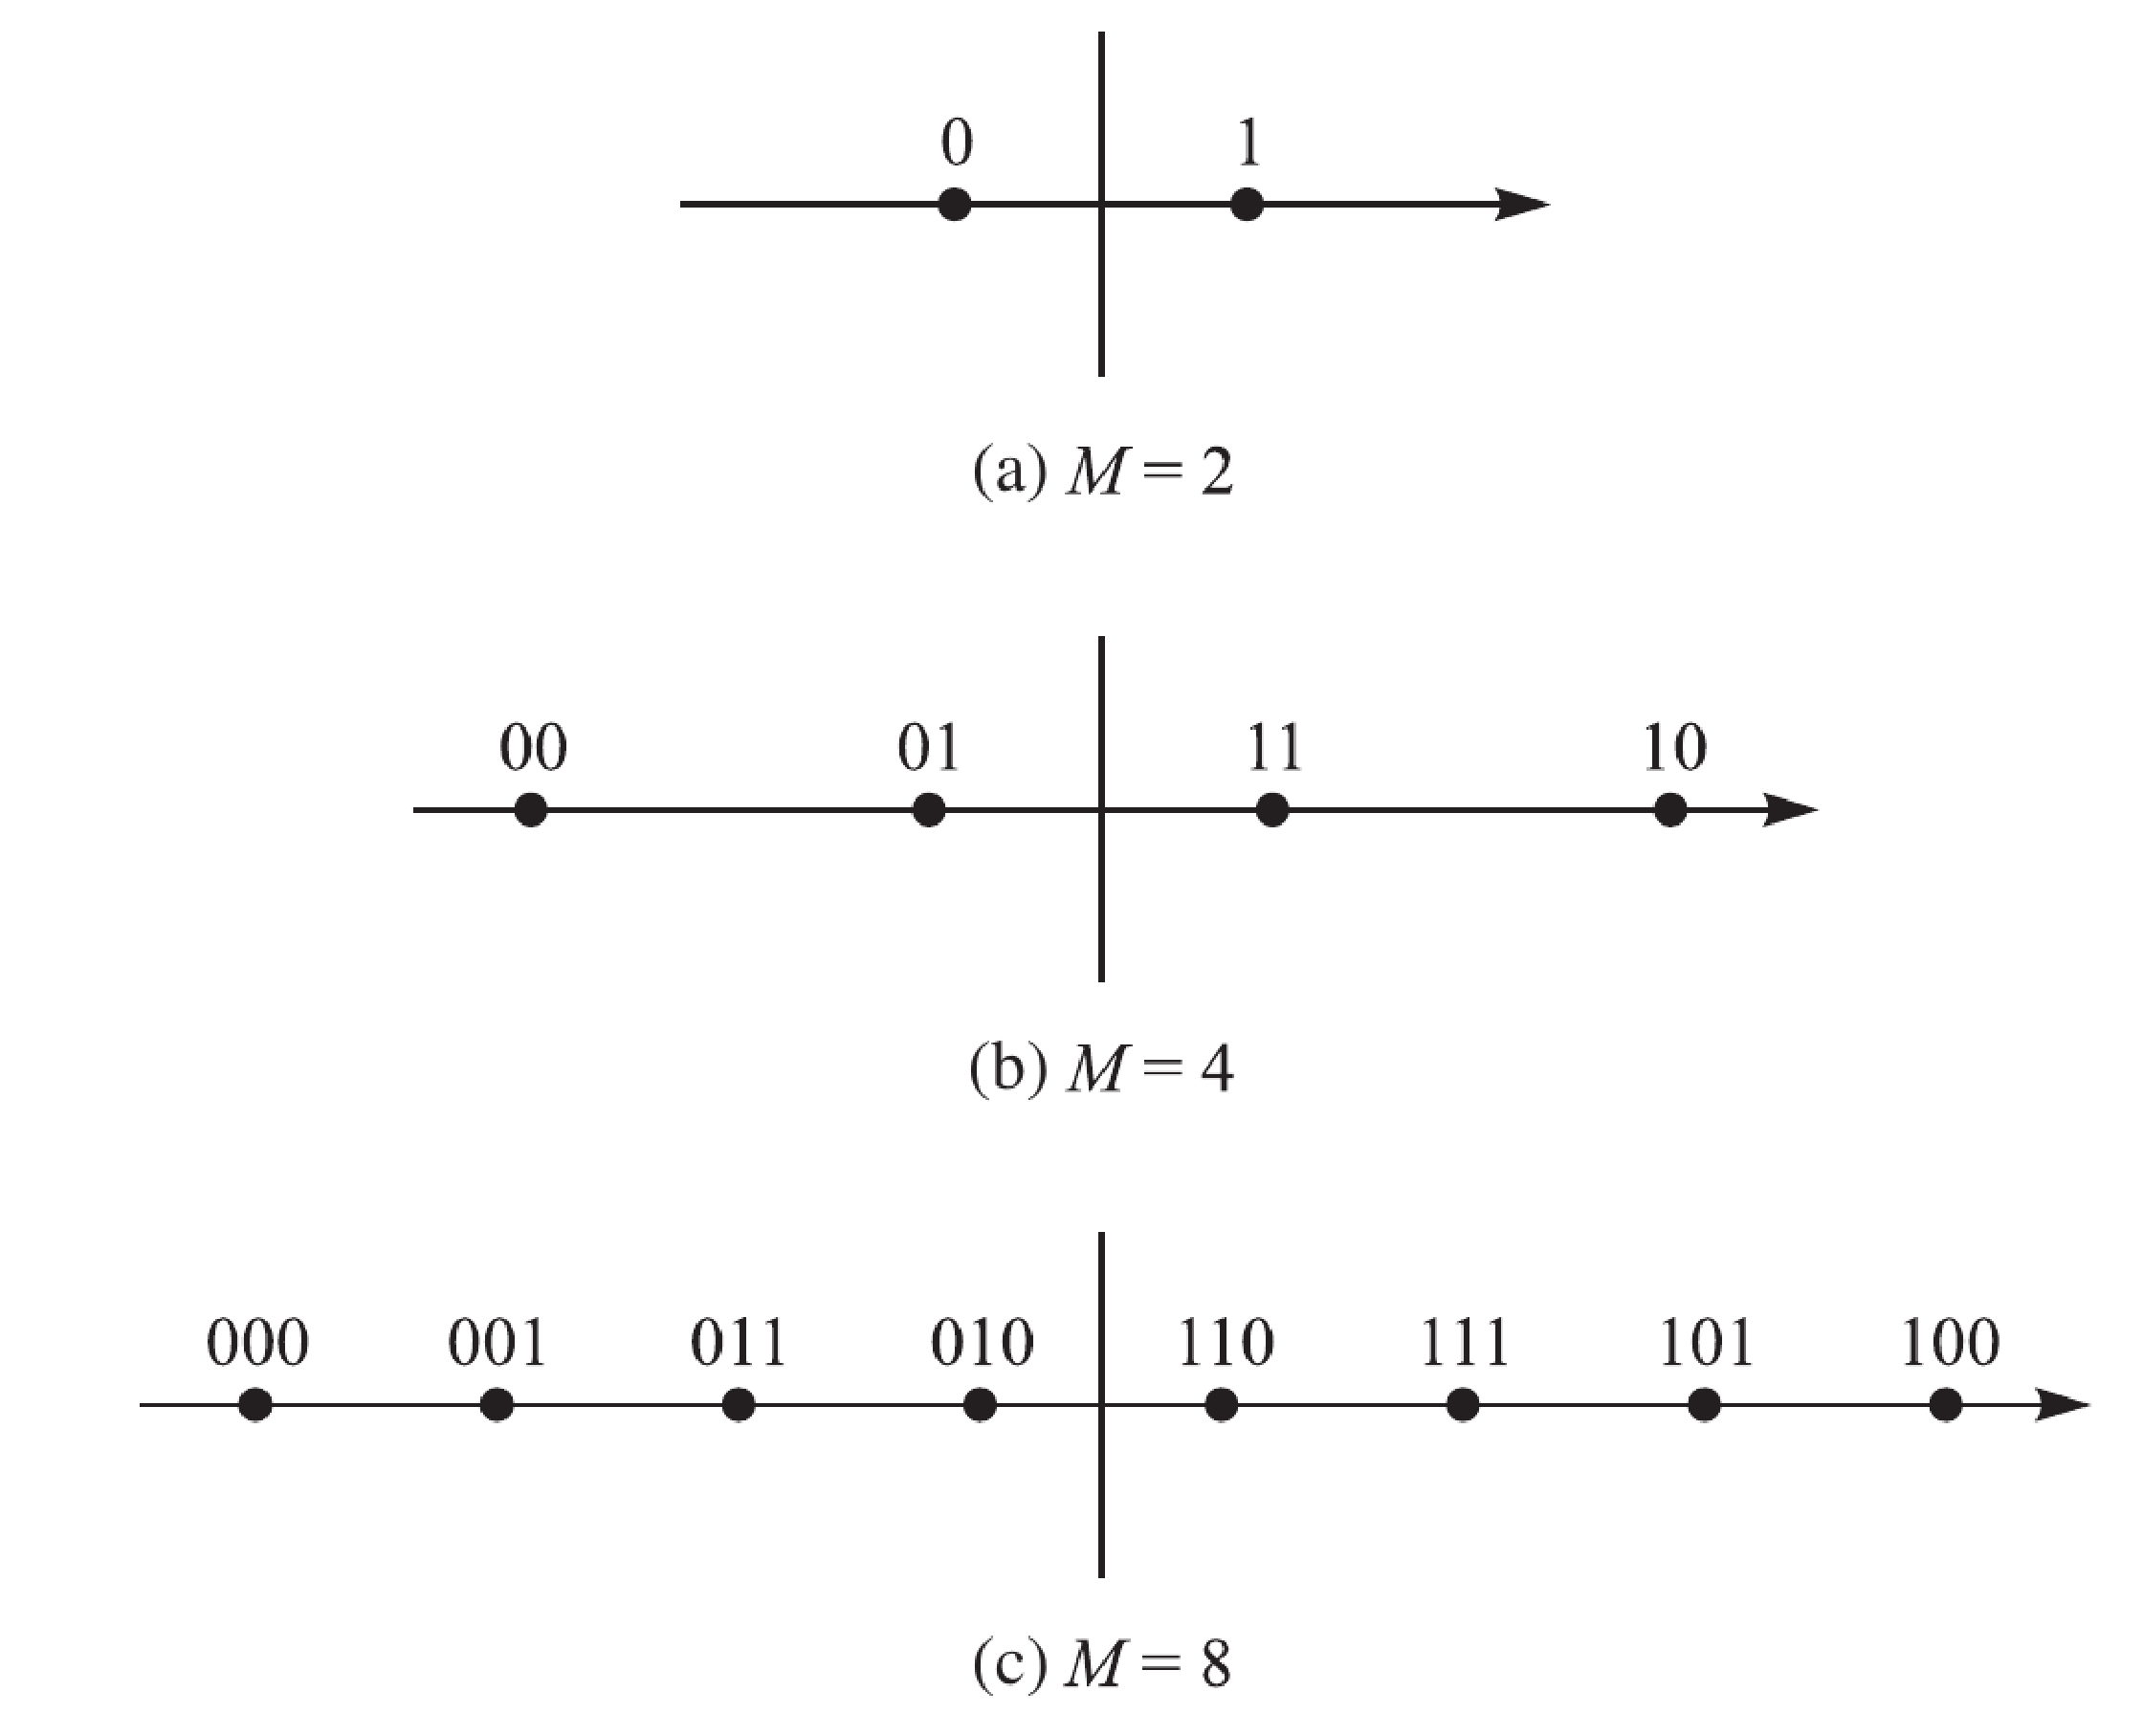
\includegraphics[width=0.6\columnwidth]{figs/4-3-1}
	  \end{center}
	\end{figure}

\end{frame}

\begin{frame}
	\frametitle{Modulação por amplitude de pulso (PAM)}

	\begin{itemize}
		\item PAM também é conhecido como Chaveamento por deslocamento de amplitude (ASK - Amplitude Shift Keying).
		\item Mapeamento dos grupos de bits (símbolos) em amplitudes de sinal:
		\begin{itemize}
			\item Pode ser feito de diversas maneiras.
			\item Mapeamento mais comum: codificação Gray, na qual sinais de amplitudes adjacentes diferem de 1 dígito binário.
			\item Motivação: erros mais prováveis causados por ruído ocorrem quando amplitudes adjacentes são incorretamente selecionadas.
			\item Na codificação Gray esse tipo de erro leva a somente 1 erro de bit na sequência de $k$ bits.
		\end{itemize}
		\item Caso particular em que $M=2$:
		\begin{itemize}
			\item Propriedade: $s_1(t) = s_2(t)$.
			\item Possuem mesma energia e coeficiente de correlação cruzada igual a -1.
			\item Sinais antipodais. 
		\end{itemize}

	\end{itemize}

\end{frame}

\begin{frame}
	\frametitle{Modulação por amplitude de pulso (PAM)}

	\begin{itemize}
		\item Distância Euclidiana entre qualquer par de pontos de sinal:
		\begin{equation*}
			d_{mn}^{(e)} = \sqrt{(s_m-s_n)^2} = \sqrt{\mathcal{E}_g/2}\, \Bigl|A_m - A_n\Bigr| = d\sqrt{2\mathcal{E}_g}\, \Bigl|m-n\Bigr|
		\end{equation*}
		\item A distância entre um par de pontos adjacentes (distância mínima) é:
		\begin{equation*}
			d_{\text{min}}^{(e)} = d\sqrt{2\mathcal{E}_g}
		\end{equation*}
		\item Sinal PAM $s_m(t)$,  para $m=1, \ldots, M$,  pode ser implementado de forma Double Side Band (DSB) ou Single Side Band (SSB):
		\begin{align*}
			s_{m, \text{DSB}}(t) &= \re\{A_m g(t) e^{j2\pi f_c t}\} \\
			s_{m, \text{SSB}}(t) &= \re\{A_m [g(t) \pm j\hat{g}(t) ] e^{j2\pi f_c t}\}
		\end{align*}
		\item Onde $\hat{g}(t)$ é a transformada de Hilbert de $g(t)$.
		\item PAM também pode ser implementado em canal sem modulação de portadora,  ou seja,  em banda base:
		\begin{equation*}
			s_m(t) = A_m g(t)
		\end{equation*}

	\end{itemize}

\end{frame}

\begin{frame}
	\frametitle{Modulação por amplitude de pulso (PAM)}

	\begin{itemize}
	 \item Sinais PAM em banda base e em banda passante:
	\end{itemize}

	
	\begin{figure}[t]
	  \begin{center}
	    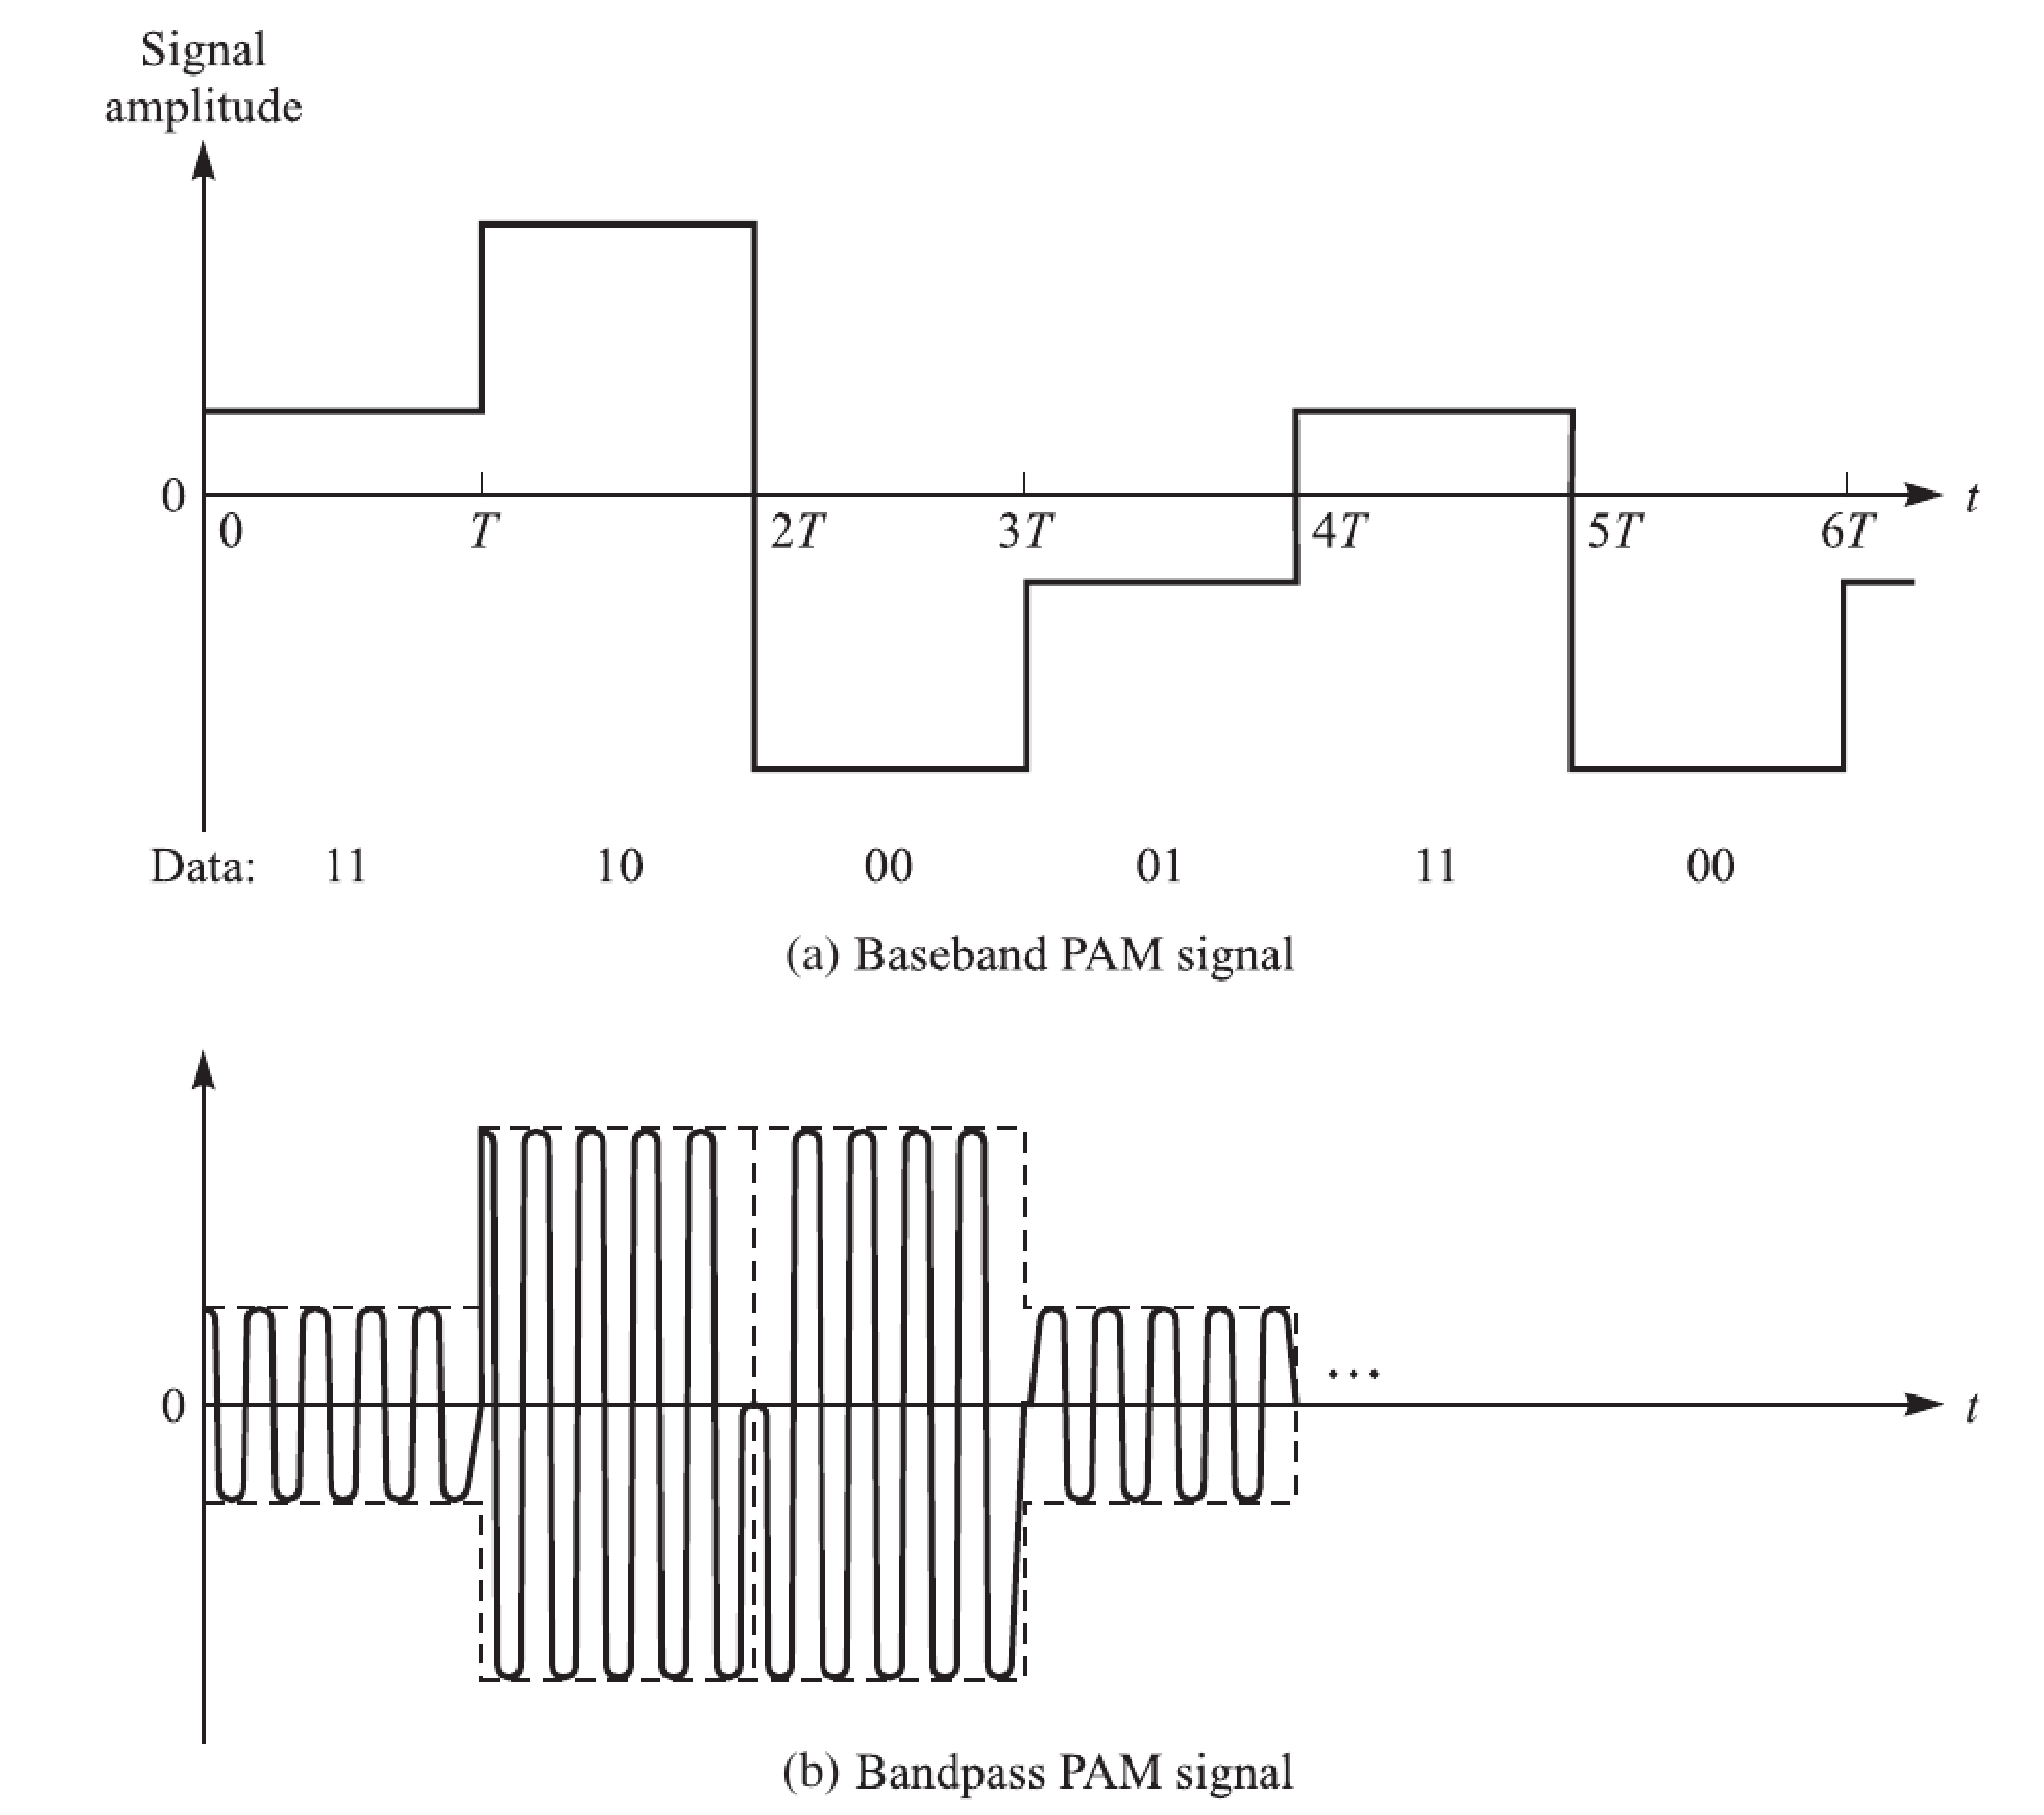
\includegraphics[width=0.6\columnwidth]{figs/4-3-2}
	  \end{center}
	\end{figure}

\end{frame}



